\documentclass[a4paper,10pt,oneside]{report}

\usepackage[french]{babel}
\usepackage[T1]{fontenc}
\usepackage[utf8]{inputenc}
% \usepackage[latin1]{inputenc}
\usepackage[dvips]{graphicx}
\usepackage{textcomp}
\usepackage[colorlinks=true,linkcolor=black,urlcolor=black]{hyperref}
\usepackage{amsmath}
\usepackage{amsfonts}
\usepackage{amssymb}
\usepackage{array}
\usepackage{geometry}
\usepackage{pifont}
\usepackage{float} 
\usepackage[svgnames]{xcolor}




\geometry{verbose,a4paper,tmargin=3cm,bmargin=3cm,lmargin=2.75cm,rmargin=2.25cm,headheight=1cm,headsep=0.825cm,footskip=1.375cm}

\title{Interpolateur interne EOS}
\date{05/09/2013}
\author{Adrien Force\\
\small{CS Systèmes d'information}}

\newcommand{\IGEN}{\textbf{\textit{EOS\_IGen}}}
\newcommand{\MESH}{\textbf{\textit{EOS\_Mesh}}}
\newcommand{\MED}{\textbf{\textit{EOS\_Med}}}
\newcommand{\IPP}{\textbf{\textit{EOS\_Ipp}}}
\newcommand{\EOS}{\textbf{\textit{EOS}}}
\newcommand{\FIELD}{\textbf{\textit{EOS\_Field}}}
\newcommand{\EFIELD}{\textbf{\textit{EOS\_Error\_Field}}}
\newcommand{\IPPl}{\textbf{\textit{\IPP\_liquid}}}
\newcommand{\IPPv}{\textbf{\textit{\IPP\_vapor}}}
\newcommand{\QI}{\textbf{\textit{EOS\_IGen\_QI}}}
\newcommand{\Cpp}[1]{\texttt{\textcolor{DimGray}{#1}}}
\newcommand{\str}[1]{\textcolor{DarkRed}{"#1"}}
\newcommand{\bdd}{base de données}
\newcommand{\ipp}{interpolateur interne d'\EOS\ }
\newcommand{\cad}{c'est à dire}
\newcommand{\pph}{plan \textbf{ph}}
\newcommand{\sgp}{segment \textbf{p}}
\newcommand{\n}{n\oe{}ud}
\newcommand{\N}{N\oe{}ud}

\newcommand{\para}[1]{(Cf. Paragraphe \ref{#1})}

\newcommand{\afair}[1]{\textcolor{red}{#1}}

\begin{document}


\maketitle \clearpage
\tableofcontents \clearpage
\chapter{Introduction}
L'interpolateur de données thermodynamiques permet aux codes clients de récupérer des données sources disponible dans EOS.
Il utilise des maillages enregistrés au préalable dans une \bdd, ce qui réduit les temps de calcul de ces données.
Les résultats ont, par contre, une moins bonne précision. Il est possible d'améliorer les valeurs calculées en ajoutant des critères de qualité,
qui induisent le raffinement des maillages.

\smallbreak
\vspace{0.3cm}
Le principe est donc de générer une \bdd\ une fois pour toutes, par l'intermédiaire du module \IGEN, puis d'interpoler dans cette 
\bdd\ les valeurs des propriétés physiques via la classe \IPP.

\begin{figure}[H]
    \center
    \includegraphics[width=1\textwidth]{EOS_interpolateur.eps}
    \caption{Schéma de principe d'EOS avec l'interpolateur interne}\label{figeos}
\end{figure}
  

\chapter{Génération d'une \bdd}
  \section{Déclaration et paramétrage d'un objet \IGEN }
    \subsection{Constructeur}\label{Constructeur}
      Il existe deux constructeurs à la classe \IGEN:
      \begin{itemize}
       \item Constructeur par défaut:\\              
       \vspace{0.3cm}
       \hspace{0.3cm} \Cpp{\IGEN\ obj\_igen;}
       
       \item Constructeur avec arguments: \\
       permet de créer un objet de la classe \IGEN\ en lui spécifiant la méthode et la référence utilisée:
       
       \vspace{0.3cm}
       
	\hspace{0.3cm}\Cpp{\IGEN\ obj\_igen(\str{EOS\_Refprop}, \str{Water});}
	
	
      \end{itemize}
      
      \subsection{Paramètres}\label{parametres}
	\subsubsection{Méthode et référence}\label{metetref}
      
	 Comme pour tout objet \EOS, il est nécessaire d'affecter à un objet de la classe \IGEN\
	 une méthode ainsi qu'une référence. Ceci peut être fait à partir des méthodes 
	 \Cpp{set\_method} et \Cpp{set\_reference} ou directement à la création de l'objet 
	 (Cf. paragraphe \ref{Constructeur}). Ces 2 paramètres définissent l'objet de la classe \EOS\
	 (attribut \Cpp{fluid} de la classe \IGEN) avec lequel sera calculé les propriétés physiques, puis généré la \bdd.
	 
	 \subsubsection{Bornes de la \bdd}\label{bornes}
	 
	 Avant la création du maillage, il est nécessaire de définir les limites en pression et en température, du domaine de la \bdd\ 
	 (pression min, pression max, température min et température max). 
	 Ces paramètres doivent être affectés à l'aide de la méthode \Cpp{set\_extremum} de la classe \IGEN.
	 Ces données, ensuite, sont traduites, afin que le maillage dépende de la \underline{pression} et de l'\underline{enthalpie}. 
	 
	 	 
	 
	 \subsubsection{Initialisation du maillage}\label{initm}
	 
	 Le maillage doit être initialisé à partir de la méthode \Cpp{make\_mesh}, possédant 3 paramètres:
	 \vspace{0.3cm}
	 \begin{itemize}
	  \item nombre de \n s en pression (obligatoire);
	  \item nombre de \n s en enthalpie (obligatoire);
	  \item niveau de raffinement maximal (optionnel).
	 \end{itemize}
	 \smallbreak
	 \vspace{0.5cm}
	 La routine \Cpp{make\_mesh} réalise les tâches suivantes:
	 \vspace{0.3cm}
	 \begin{itemize}
	  \item Calcul de l'enthalpie minimum et de l'enthalpie maximum du maillage;
	  \item Instanciation de 2 objets de la classe \MESH:
	  \begin{itemize}
	    \item[\ding{213}]Attribut \Cpp{mesh\_ph} de la classe \IGEN: maillage surfacique pression-enthalpie (\pph);
	    \item[\ding{213}]Attribut \Cpp{mesh\_p}  de la classe \IGEN: segment en pression (\sgp);
	  \end{itemize}
	  \item Création d'une \bdd\ temporaire;
	  \item Affectation de l'attribut \Cpp{obj\_Ipp} objet de la classe \EOS.
	 \end{itemize}
      
      \section{Critères de qualité}\label{qualite}
	\subsection{Déclaration}
	Les critères de qualité se définissent à l'aide de la méthode \Cpp{set\_quality}, via 4 paramètres:
	\vspace{0.3cm}
	\begin{itemize}
	 \item \Cpp{property}: propriété physique sur laquelle s'applique le critère de qualité;
	 \item \Cpp{type}: méthode de calcul de la qualité;
	 \item \Cpp{is\_abs}: norme définissant si la qualité est calculée en relatif ou en absolu\\ (0: relatif; 1: absolu);
	 \item \Cpp{limit\_qi}: Limite haute (seuil de qualité) que doit respecter l'écart entre
	 les calculs de la propriété avec l'interpolateur (\IPP) et les calculs de la propriété avec la méthode \EOS\ de référence.
	\end{itemize}
	\smallbreak
	\vspace{0.5cm}
	Pour un maillage il peut y avoir un nombre indéfini de critères de qualité, 
	à chaque appel de la méthode \Cpp{set\_quality} un nouvel objet de la classe \QI\ est créé, puis ajouté à 
	l'attribut \Cpp{qualities} de la classe \IGEN.
	
	
      \subsection{Principe}
      
      Les critères de qualité sont ce qui permet d'accorder la validité d'une maille
      ainsi que le maillage dans ça globalité.
      La qualité d'un maillage est estimée à l'aide de la méthode \Cpp{compute\_qualities} de la classe \IGEN.
      
      \subsubsection{calcul de la qualité}
      
      La qualité s'applique maille/maille, de façon indépendante.
      Ce sont les critères de qualité qui vont, dans le cas d'un raffinement
      local \para{raflocal}, déterminer si la maille a besoin d'être raffinée.
      \smallbreak\vspace{0.3cm}
      Aujourd'hui, pour calculer la qualité des mailles, une seule méthode est implémentée.
      La méthode se détermine, en affectant le mot clé \str{centre} au paramètre \Cpp{type},
      celui-ci indique que la propriété est calculée, via l'interpolateur et via la méthode de référence,
      au centre de la maille. Puis la différence de ces deux résultats est comparée au seuil, si elle est inférieure la maille
      est dite valide (en erreur sinon). En relatif la différence est divisée par le résultat de la méthode de référence.

      
      \subsubsection{Implémentation future}
      \begin{enumerate}
       \item D'autre méthodes de calcul de la qualité pourront être implémentées:
       \vspace{0.3cm}
       \begin{itemize}
	 \item \str{multipoint}: écart entre une grandeur interpolée et la grandeur d’origine en 9 points des mailles;
	 \item \str{d\_rho}: écart entre dérivée numérique de la masse volumique à partir des grandeurs interpolées et la valeur interpolées;
	 \item \str{d\_h}: écart entre la dérivée numérique de l’enthalpie en fonction de la température à pression constante.
       \end{itemize}
       \item Un calcul \EOS\ peut retourner une erreur, pour différentes raisons, celles-ci ne sont pas décrites ici.  
	Il est donc, possible que certains \n s d'un maillage soient dans un domaine ``non valide''.
	Ainsi, lorsqu'une maille a ces quatre \n s dans un domaine ``non valide'', il n'y aucune nécessité de la raffiner, 
	la validité des \n s pourrait être un paramètre de la validité de la maille.
      \end{enumerate}
	 
    \section{Raffinement}\label{raf}
    
    Deux types de raffinement sont implémentés dans la classe \IGEN, le raffinement global et le raffinement local. 
    Un raffinement s'arrête lorsque toutes les mailles sont valides \para{qualite}
    ou que son niveau maximum de raffinement est atteint \para{initm}.
    
    \subsection{Raffinement global}
    Le raffinement global permet, lorsqu'un critère de qualité n'est pas respecté de raffiner le maillage dans sa globalité (méthode \Cpp{make\_global\_refine}).
    Ainsi, par niveau de raffinement, chaque maille est divisée en quatre parties égales. 
    Cette méthode est peu optimisée car lorsqu'une seule maille est en erreur tout le maillage est raffiné.
    
    \subsection{Raffinement local}\label{raflocal}
    
    Le raffinement local a été implémenté dans le but de raffiner seulement les mailles dont les critères de qualité ne sont pas respectés.
    Cependant la démarche d'un raffinement local pose un problème de continuité des valeurs dans le \pph, en effet une propriété calculée à la 
    frontière de 2 mailles côte à côte, de taille différente, peut ne pas donner le même résultat d'une maille à l'autre (Cf Annexe \ref{cnt}). 
      
      \subsubsection{Principe}
      Le raffinement se réalise via la méthode \Cpp{make\_local\_refine} de la classe \IGEN.
      Cette méthode réalise les tâches suivante:
      \vspace{0.3cm}
      \begin{itemize}
       \item Calcul de la qualité: méthode \Cpp{compute\_qualities} de la classe \IGEN;
       \item Création des nouveaux \n s des maillages (\pph\ et \sgp): méthode \Cpp{add\_local\_nodes}, classe \MESH;
       \item Ajout des \n s de continuité (plan \textbf{ph}): méthode \Cpp{add\_continuity\_nodes}, classe \MESH;
       \item écriture d'une \bdd\ temporaire: méthode \Cpp{write\_tempory\_med}, classe \IGEN.
      \end{itemize}
      \vspace{0.5cm}
      
      \subsubsection{Création de \n s}
	\begin{description}
	 \item[\textbullet] \textbf{\sgp:}
	 \smallbreak
	 La réalisation d'un raffinement local, sur le \sgp, ne pose aucune difficulté:
	  \vspace{0.3cm}
	  \begin{itemize}
	  \item Ajout d'un point au centre des segments locaux dont la qualité n'est pas respecter;
	  \item renumérotation des \n s du \sgp\ global.
	  \end{itemize}
	 
	 \vspace{0.3cm}
	 \item[\textbullet] \textbf{\pph:}
	   \smallbreak
	   Pour effectuer un raffinement local, dans le \pph, deux types de maillage sont utilisés:
	   \vspace{0.3cm}
	   \begin{itemize}
	    \item maillage global: maillage fictif où toutes les mailles sont raffinées. 
	    Ce maillage est représenté par l'attribut \Cpp{node\_glb} qui décrit les \n s par un entier (Cf. Figure \ref{nodeglb}):
	      \begin{itemize}
		\item[\ding{213}] \Cpp{node\_glb[i] = 0}: \n s fictifs; 
		\item[\ding{213}] \Cpp{node\_glb[i] = 1}: \n s du maillage initial et \n s au centre d'une maille précédemment raffinée;
		\item[\ding{213}] \Cpp{node\_glb[i] = 2 ou 9}: \n s d'une maille raffinée, calculés sur un segment à \textbf{p} constant 
		(2: en cours de raffinement, 9: niveau de raffinement antérieur);
		\item[\ding{213}] \Cpp{node\_glb[i] = 3 ou 8}: \n s d'une maille raffinée, calculés sur un segment à \textbf{h} constant 
		(3: en cours de raffinement, 8: niveau de raffinement antérieur);
		\item[\ding{213}] \Cpp{node\_glb[i] = 4}: \n s au centre d'une maille en cours de raffinement;
	      \end{itemize}
	    \vspace{0.3cm}
	    \item maillage réel: maillage avec seulement les mailles en erreurs raffinées (maillage stocké dans la \bdd). 
	    Ici les \n s sont décrits par leurs valeurs en \textbf{p}, en \textbf{h} ainsi que leur type (Cf. \textbf{Continuité} paragraphe \ref{continuite}).
	   \end{itemize}

	 \begin{figure}[H]
	  \center
	  \includegraphics[width=0.75\textwidth]{schema_2d_ndglb.eps}
	  \caption{Exemple d'un maillage global, représentation graphique du vecteur \Cpp{node\_glb}}\label{nodeglb}
	 \end{figure}
	 
	 Le raffinement local dans le \pph, est réalisé selon l'algorithme suivant:
	 \vspace{0.3cm}
	 \begin{itemize}
	  \item Création de l'équivalence mailles globales - mailles réelles;
	  
	  \item Calculs du nombre de \n s et du nombre de mailles à ajouter pour ce niveau de raffinement;
	  
	  \item Détermination de la position des nouveaux \n s réels dans le maillage global;
	  
	  \item Affectation à chaque \n s des valeurs \textbf{h} et \textbf{p};
	  
	  \item Spécification du vecteur d'équivalence \n s globaux - \n s réel;
	  
	  \item Détermination de la correspondance des mailles globales aux 4 \n s qui l'entourent (attribut \Cpp{med\_to\_node} de la classe \MESH).
	 \end{itemize}

	 
	\end{description}

	Il est à noter qu'un critère de qualité avec une propriété calculée dans le \pph\ 
	impose un raffinement seulement dans le maillage \textbf{ph} 
	et respectivement pour une propriété du \sgp.

      
      \subsubsection{Continuité}\label{continuite}
      
      La continuité est construite à partir du maillage global, sur lequel sont ajoutés les \n s de continuité:
      \begin{itemize}
       \item placement des \n s existant (\n s de continuités et \n s réels) dans le nouveau maillage global;
        
       \item Affectation des valeurs \textbf{h} et \textbf{p} (Attribut \Cpp{continuity\_h} et \Cpp{continuity\_p}, de la classe \MESH)
       et ajout au maillage global des nouveaux \n s de continuité (Attribut \Cpp{continuity\_node} de la classe \MESH):
	\begin{itemize}
	\item[\ding{213}] \Cpp{continuity\_node[i] = 0}: \n s réels ou fictifs;
	\item[\ding{213}] \Cpp{continuity\_node[i] = 1 ou 7}: \n s de continuité à \textbf{p} constant;
	\item[\ding{213}] \Cpp{continuity\_node[i] = 2 ou 8}: \n s de continuité à \textbf{h} constant;
	\item[\ding{213}] \Cpp{continuity\_node[i] = 3 ou 9}: \n s de continuité aux centres des mailles;
	\end{itemize}
       \vspace{0.3cm}
       \item Spécification des \n s dans le maillage réel (attribut \Cpp{type\_of\_node}, de la classe \MESH):
	\begin{itemize}
	  \item[\ding{213}] \Cpp{type\_of\_node[i] = 0}: \n s réels;
	  \item[\ding{213}] \Cpp{type\_of\_node[i] = 1}: \n s de continuité à \textbf{p} constant;
	  \item[\ding{213}] \Cpp{type\_of\_node[i] = 2}: \n s de continuité à \textbf{h} constant;
	  \item[\ding{213}] \Cpp{type\_of\_node[i] = 3}: \n s de continuité aux centres des mailles;
	\end{itemize}
       \vspace{0.3cm}
       \item Modification l'attribut \Cpp{med\_to\_node} avec la prise en compte des \n s de continuité;
       \item Détermination de la correspondance des \n s de continuité aux 2 \n s qui l'entourent 
       (Attribut \Cpp{continuity\_to\_node} de la classe \MESH).
      \end{itemize}

    \section{Ecriture d'une \bdd}\label{ebdd}
    
    Une \bdd\ est générée au format ``MED FICHIER''\footnote{Pour le moment, les fichiers sont produit au format ``MED-2''}.
    Une fois les paramètres définis, pour générer une \bdd, il suffit de faire 
    appel à la méthode \Cpp{write\_med} de la classe \IGEN.
    Ce programme utilise plusieurs méthodes de la classe \MED\ et écrit ainsi le fichier de
    la \bdd, enregistré avec une extension ``.med''. 
    De plus le fichier index.eos est mis à jour, pour que la nouvelle \bdd\ soit reconnue par \EOS\ et utilisable par l'interpolateur.
    
      \subsection{Nom du fichier de la \bdd}
      
      Il y a deux possibilités pour définir le nom du fichier dans lesquels la \bdd\ est sauvegardée:
      \vspace{0.3cm}
      \begin{itemize}\itemsep0.3cm
       \item Formatage par défaut:
       \smallbreak
       \begin{tabbing}
       \hspace{-0.5cm} \= \kill
       \> \Cpp{\str{méthode}.\str{référence}.ph\_field.p\str{pmin}\_\str{pmax}.h\str{hmin}\_\str{hmax}.p\_field.p\str{pmin}\_\str{pmax}}
       \end{tabbing}
       
       \item Entrer un nom: à l'aide de la méthode \Cpp{set\_file\_med\_name} de la classe \IGEN, exemple:
       
       \Cpp{
       \begin{tabbing}
       \hspace{0.5cm} \= \kill
       \> AString file\_name=\str{raffinement\_local};\\
       \> obj\_igen.set\_file\_med\_name(file\_name);
       \end{tabbing}
       }
      \end{itemize}
      \vspace{0.5cm}
      
      
      \subsection{Enregistrement du domaine et des propriétés}
      
      Que ce soit pour la création de la \bdd\ finale ou d'une \bdd\ temporaire, le domaine d'étude ainsi que les propriétés
      physiques sont enregistrés à partir de la méthode \Cpp{make\_properties} de la classe \IGEN. 
      L'écriture dans la \bdd\ s'effectue, de façon similaire pour le \pph\ et le \sgp, selon les étapes suivantes:
      \vspace{0.3cm}
      \begin{itemize}
       \item Ajout d'un maillage\footnote{Ici 3 maillages différents peuvent être enregistrés 
	  \begin{itemize}
	   \item \pph: \str{ph\_domain}
	   \item saturation: \str{sat\_domain} (\sgp)
	   \item spinodal: \str{lim\_domain} (\sgp)
          \end{itemize}
	}: méthode \Cpp{add\_Maillage} de la classe \MED
       \item Ajout du domaine (valeurs en p et en h des \n s): \Cpp{add\_Nodes} de la classe \MED;
       \item Création du vecteur de connectique, permettant le repérage d'un point dans le maillage
       (Cf. paragraphe \ref{connectique}). Trois méthodes de la classe \MED\ sont utilisées selon les circonstances:
	\begin{itemize}
	  \item[\ding{213}] \Cpp{add\_Connectivity\_NoRef\_2D}: \pph\ sans raffinement (ou raffinement global);
	  \item[\ding{213}] \Cpp{add\_Connectivity\_Refine\_2D}: \pph\ avec raffinement local;
	  \item[\ding{213}] \Cpp{add\_Connectivity\_1D}: \sgp.
	\end{itemize}
       \vspace{0.3cm}
       \item Calcul des propriétés une à une: méthode \Cpp{compute} de la classe \EOS\ (Cf. paragraphe \ref{properte});
       \item Stockage des propriétés une à une: \Cpp{add\_Champ\_Noeud} de la classe \MED;
       \item Enregistrement des erreurs par propriété et par \n: méthode \Cpp{add\_ErrChamp\_Noeud} de la classe \MED.
      \end{itemize}
      
      
      \section{Calcul des propriétés}\label{properte}
      
      Le calcul des propriétés s'effectue par champs, via les méthodes de type ``\Cpp{compute}'' des classes \EOS\ (Cf. paragraphe \ref{metetref}). 
      Les résultats sont directement stockés dans une \bdd\ temporaire ou dans la \bdd\ finale.
      
      \subsection{Champs}
       \subsubsection{Champs dans le \pph}
       Dans le \pph, il existe deux champs, les valeurs en \textbf{p} et les 
       valeurs en \textbf{h} correspondant aux \n s du maillage. Les champs ont une taille 
       initiale = \textbf{nombre de valeurs en p} * \textbf{nombre de valeurs en h}.
       Après raffinement local, la taille des champs ne peut plus s'exprimer par une formule étant donné la complexité du maillage.
       
       \subsubsection{Champ du \sgp} 
       \n s du \sgp.
       
       \subsection{Calcul des propriétés aux \n s de continuité }
       Afin de garantir la continuité dans tout le maillage,
       les propriétés à chaque \n\ de continuité sont déterminées par la demi somme des valeurs des 2 \n s qui l'entourent (Cf. Figure \ref{1cont}).
       \begin{figure}[H]
	\center
	\includegraphics[width=0.66\textwidth]{schema_2d_ct.eps}
	\caption{Exemple d'un maillage réel avec continuité.}\label{1cont}
       \end{figure}
       Dans certaines configurations, la continuité impose de séparer en 4, une maille moins raffinée,
       ce qui induit 3 \n s de continuité (Cf. Figure \ref{2cont}).
       Par choix, les propriétés des \n s de continuité aux centres des mailles, sont directement calculées par \EOS.
       \begin{figure}[H]
	\center
	\includegraphics[width=0.66\textwidth]{schema_2d_2ct.eps}
	\caption{Exemple d'un maillage réel avec continuité croisée.}\label{2cont}
       \end{figure}
     
      
  
   \clearpage    
 
      

\clearpage


\section{Description des classes}
  \subsection{Ordre d'appel}
    La création d'une \bdd\ doit respecter les régles d'appel suivantes:
    \subsubsection{Création d'un objet \IGEN\ \para{Constructeur}}
      \begin{itemize}
       \item[\ding{0}] En début de programme
       \item[\ding{0}] \Cpp{\IGEN\ obj\_igen;}
       \item[\ding{0}] \Cpp{\IGEN\ obj\_igen(method, reference);}
      \end{itemize}
    \subsubsection{Paramètres \para{parametres}}
      \begin{itemize}
	\item[\ding{0}] Doit être mis avant la création des maillages
	\item[\ding{0}] \Cpp{obj\_igen.set\_method(method);}
	\item[\ding{0}] \Cpp{obj\_igen.set\_extremum(pmin,pmax,Tmin,Tmax);}
      \end{itemize}
    \subsubsection{Création des maillages \para{initm}}
      \begin{itemize}
	\item[\ding{0}] \Cpp{obj\_igen.make\_mesh(nb\_p, nb\_h, level\_max);}
      \end{itemize}
    \subsubsection{Critères de qualités \para{qualite}}
      \begin{itemize}
	\item[\ding{0}] Doit être placé avant le raffinement, 
	\item[\ding{0}] plusieurs critères de qualité peuvent être définis
	\item[\ding{0}] \Cpp{obj\_igen.set\_quality(property,type,is\_abs,limit\_qi);}
      \end{itemize}
    \subsubsection{Raffinement des maillages \para{raf}}
      \begin{itemize}
	\item[\ding{0}] Lorsque l'objet \IGEN\ est complètement paramétré
	\item[\ding{0}] \Cpp{obj\_igen.make\_global\_refine();}
	\item[\ding{0}] \Cpp{obj\_igen.make\_local\_refine();}
      \end{itemize}
    \subsubsection{Ecriture de la \bdd\ \para{ebdd}}
      \begin{itemize}
	\item[\ding{0}] Optionnel
	\item[\ding{0}] \Cpp{obj\_igen.set\_file\_med\_name(file\_med\_name);}
	\item[\ding{0}] Dernier appel 
	\item[\ding{0}] \Cpp{obj\_igen.write\_med();}
      \end{itemize}
      
    \clearpage
      
  \subsection{Classes et attributs}
    La Figure \ref{uml_att} présente la hiérarchie des classes, ainsi que le descriptif des attributs, sous la forme d'un diagramme UML:
    \begin{figure}[H]
      \center
      \includegraphics[width=1.0\textwidth]{Eos_IGen_att.eps}
      \caption{Diagramme UML des classes permettant la génération de \bdd}\label{uml_att}
    \end{figure}
    
    

\chapter{Interpolation des données d'une base}
  \section{Généralités}\label{general}
    L'utilisation de l'\ipp s'effectue de la même façon que les autres méthodes d'\EOS,
    la déclaration se fait à l'aide de la méthode \str{\IPP}
    et d'une référence correspondant au nom du fichier au format ``med'', contenant la \bdd, exemple:
    \vspace{0.3cm}
    \begin{itemize}
     \item[\ding{0}] \Cpp{\EOS\ obj\_ipp(\str{\IPP}, \str{med\_file});}
    \end{itemize}
    \vspace{0.5cm}
    
    Avec ce constructeur toutes les propriétés de la \bdd\ sont chargées.
    \smallbreak
    \vspace{0.2cm}
    A noter, il est possible de faire un chargement sélectif, en spécifiant une liste de propriétés à l'instanciation de l'objet \EOS: 
    
    \vspace{0.3cm}
    \begin{itemize}
      \item[\ding{0}] \Cpp{Strings list(3);}
      \item[\ding{0}] \Cpp{list[0] = \str{T\_sat};}
      \item[\ding{0}] \Cpp{list[1] = \str{rho};}
      \item[\ding{0}] \Cpp{list[2] = \str{Cp};}
      \item[\ding{0}] \Cpp{\EOS ipp(\str{\IPP},\str{med\_file},list);}
    \end{itemize}
    \vspace{0.5cm}
     
    Le module de l'\ipp\ contient une classe principale \IPP\ ainsi que 2 classes dérivées, une pour la phase liquide et une pour la phase vapeur,
    respectivement: \IPPl\  et \IPPv. Ces 2 classes filles contiennent une surcharge des fonctions ``compute'' dans le plan \textbf{pT}.


    \section{Chargement des données de la classe \IPP}
       
    \subsection{Entête}
    L'entête du fichier med (\Cpp{header}), permet notemment au 
    programme de récupérer le couple méthode/référence, utilisé pour créer la \bdd.
    Ces valeurs sont, ensuite, affectées sous forme de chaînes de caractères, aux attributs \Cpp{base\_method} et \Cpp{base\_reference}.
    
    \subsection{Maillages}\label{maillages}
    Les maillages enregistrés dans la \bdd\ possèdent les dénominations suivantes:
    \vspace{0.3cm}
    \begin{itemize}
      \item[\ding{192}] \pph: \str{ph\_domain};
      \item[\ding{193}] saturation: \str{sat\_domain} (\sgp);
      \item[\ding{194}] spinodal: \str{lim\_domain} (\sgp).
    \end{itemize}
    \vspace{0.5cm}
    
    Cet aiguillage permet l'affectation des attributs, respectif à chaque maillage:
    \vspace{0.3cm}
    \begin{itemize}
      \item Valeurs des noeuds: \Cpp{n\_p\_ph} \ding{192}, \Cpp{n\_h\_ph} \ding{192}, \Cpp{n\_p\_satlim} \ding{193}\ding{194};
      \item Domaine d'étude: \Cpp{nodes\_ph} \ding{192}, \Cpp{nodes\_sat} \ding{193}, \Cpp{nodes\_lim} \ding{194};
      \item Vecteur de connectique (Cf. paragraphe \ref{connectique}):
      connect\_ph \ding{192}, connect\_sat \ding{193}, connect\_lim \ding{194};
      \item Numérotation des cellules: index\_conn\_ph \ding{192}.
    \end{itemize}
    \vspace{0.5cm}
    
    \subsection{données scalaires}
    Les données scalaires décrivant les maillages de la \bdd\ sont affectées aux attributs suivants:
    \vspace{0.3cm}
    \begin{itemize}
      \item \Cpp{pmin}: Pression minimum
      \item \Cpp{pmax}: Pression maximum
      \item \Cpp{hmin}: Enthalpie minimum
      \item \Cpp{hmax}: Enthalpie maximum
      \item \Cpp{tmin}: Température minimum
      \item \Cpp{tmax}: Température maximum
      \item \Cpp{delta\_p\_f}: Ecart en pression de la maille la plus raffinée\footnote{Taille en pression ou en enthalpie 
      d'une maille du maillage global Cf. paragraphe \ref{raflocal}\label{delta}}
      \item \Cpp{delta\_h\_f}: Ecart en enthalpie de la maille la plus raffinée\textsuperscript{ \ref{delta}}
      \item \Cpp{tcrit}: Température critique du fluide
      \item \Cpp{pcrit}: Pression critique du fluide
      \item \Cpp{hcrit}: Enthalpie critique du fluide
    \end{itemize}
    \vspace{0.5cm}
    
    \subsection{propriétés}
    L'\ipp charge les valeurs des propriétés de la \bdd\ med en mémoire,
    soit dans son integralité soit par sélection définie par l'utilisateur (Cf. Paragraphe \ref{general}).
    \smallbreak\vspace{0.3cm}
    Toutes les valeurs, des propriétés chargées, aux \n s des maillages
    sont stockées dans le tableau \Cpp{all\_prop\_val}\footnote{La nécessité de stocker les tableaux
    de valeurs compris dans les champs, vient du choix de développement qu'à la création d'un objet de la classe \FIELD,
    ce tableau doit lui être passé par référence.\label{field}}.
    Par contre les champs des propriétés sont affectées avec la distinction du maillage sur lequel ils s'appliquent 
    (Cf. paragraphe \ref{maillages}). Il y a donc 3 attributs à la classe \IPP\ comprenant ces champs:
    \vspace{0.3cm}
    \begin{itemize}
      \item \Cpp{val\_prop\_ph} \ding{192}
      \item \Cpp{val\_prop\_sat} \ding{193}
      \item \Cpp{val\_prop\_lim} \ding{194}
    \end{itemize}
    \vspace{0.5cm}
    
    \subsection{Erreurs}
    Les erreurs, considérés ici, proviennent de la méthode avec laquelle a été créée la \bdd.
    Elles sont stockées sous forme d'un tableau, par propriété, qui contient l'erreur à chaque \n\ du maillage.
    Cependant, lors du chargement, un traitement est effectué pour que l'erreur soit étendu à la maille,
    car si un des \n s de la maille est faux alors toutes les valeurs interpolées dans cette maille sont en erreur.
    \smallbreak\vspace{0.3cm}
    De la même façon que pour les propriétés il y a 1 attribut qui stocke tous les tableaux des erreurs 
    relevées\footnote{Même fonctionnement de la classe \EFIELD\ que la classe \FIELD, voir note \ref{field}} (\Cpp{all\_err\_val})
    et 3 attributs déffinissant les champs d'erreurs dans les maillages:
    \vspace{0.3cm}
    \begin{itemize}
      \item \Cpp{err\_cell\_ph} \ding{192}
      \item \Cpp{err\_segm\_sat} \ding{193}
      \item \Cpp{err\_segm\_lim} \ding{194}
    \end{itemize}
    \vspace{0.5cm}
   
   
   \section{Connectique}\label{connectique}
   
   Etant donné l'irrégularité des tailles de mailles, due au raffinement local, le repérage d'un point dans un maillage, est réalisé à partir
   de la succession de vecteurs d'indices d'équivalence,
   d'un repère à un autre, c'est ce qui est appelé connectique. Elle assure, lors d'un calcul d'une propriété en un point quelconque du maillage, 
   que l'interpolation est réalisée avec les points rééls ou de continuité les plus proches.
   \vspace{0.3cm}
   \begin{itemize}
     \item[\textbullet] \textbf{Le positionnement d'un point sur le \sgp:}\\
     Le positionnement d'une valeur en pression ($p$), est réalisé en récupérant le premier indice ($i$) des vecteurs
     \Cpp{connect\_sat} ou \Cpp{connect\_lim}, pour lequel la valeur \Cpp{nodes\_sat} ou \Cpp{nodes\_lim} respectivement, est supérieure à $p$.
     Les indices des valeurs de \Cpp{nodes\_sat} ou \Cpp{nodes\_lim}, sont donc $i-1$ et $i$.
%      \smallbreak\vspace{0.3cm}
%      L'intérêt de passer, ici, par un vecteur de
%      connectique intermédiaire reste à determiner.
     \smallbreak\vspace{0.3cm}
     \item[\textbullet] \textbf{Le positionnement d'un point dans le \pph:}\\
      Lors du chargement des données, l'attribut vecteur \Cpp{fnodes2phnodes}, de la classe \IPP,
      est affecté pour chaque maille du maillage global (mailles fictives, Cf. Paragraphe \ref{raflocal})
      par l'indice du premier \n\ de cette maille (plus petites valeurs de \textbf{p} et de \textbf{h}).
      \smallbreak\vspace{0.3cm}
      Lors du calcul d'une propriété en un point $i$,
      le point est positionné, dans un premier temps, dans la maille fictive ($m$),
      à l'aide des données \Cpp{delta\_p\_f} et \Cpp{delta\_h\_f}. 
      Puis dans un second temps l'indice du premier \n\ de $m$ est récupéré, avec \Cpp{i=fnodes2phnodes[m]}.
      Enfin les indices des 4 \n s de la maille encadrant le point, correspondent aux valeurs comprises dans l'intervalle:
      \begin{align*}
      [connect\_ph[i];connect\_ph[i+3]];
      \end{align*}
      Avec, \Cpp{connect\_ph[i]} vecteur de correspondance \n s~fictifs/\n s~réels.
      \smallbreak\vspace{0.3cm}
   
   \end{itemize}
   \vspace{0.5cm}
   
   
   \section{Interpolation}
   
    \subsection{Calculs des propriétés}
    
    Selon la propriété calculée, les grandeurs peuvent être interpolées directement ou déduites:
    
    \subsubsection{Grandeurs interpolées directement}
    \begin{itemize}
      \item La température de saturation (\textbf{T\_sat});
      \item Toutes les dérivées par rapport à \textbf{p};
      \item Les enthalpies dans le domaine spinodal et dans le plan \textbf{pT} \textbf{(h\_l\_lim}, \textbf{h\_v\_lim}, \textbf{h\_pT});
      \item Toutes les propriétés du \pph;
      \item Toutes les dérivées des propriétés du \pph.
    \end{itemize}
    A noter, qu'aucune cohérence n'est faite dans l'interpolateur, entre les grandeurs et leurs dérivées.
    
    \subsubsection{Grandeurs déduites}
    \begin{itemize}
      \item Toutes les propriétés dans le plan \textbf{pT}, en dehors de \textbf{h\_pT};
      \subitem Le calcul dans le plan \textbf{pT}, par exemple pour la propriété \textbf{rho}, passe par l'intermédiaire suivant:
      \begin{align*}
      &rho(p,T) = rho(p,h)\\
      &\text{Avec, } h = h(p,T)\\
      &=> T = T(p,h)
      \end{align*}
      
      \item Toutes propriétés dans le domaine de saturation, en dehors des dérivées et de \textbf{T\_sat}.
      \subitem Le calcul des grandeurs à saturation passe par plusieurs calculs intermédiaires, par exemple pour propriété \textbf{rho\_l\_sat}:\\
       \begin{align*}
	&rho^l_{sat}(p) = rho(p,h^l_{sat})\\
	&\text{Avec, } h^l_{sat} = h^l(p,T_{sat})\\
	&=> T_{sat} = T(p,h^l_{sat}) = T(p,h^v_{sat})
       \end{align*}
    \end{itemize}
    A noter, les grandeurs détuites assurent la cohérence entre les propriétés du \pph\ et les grandeurs de saturation.

    \subsection{Interpolation}
    \begin{itemize}
      \item[\textbullet] L'interpolation des valeurs sur le \sgp\ se fait de façon linéaire.
      \item[\textbullet] Dans le \pph\ l'interpolation est dite ``bilinéaire'':
       \smallbreak\vspace{0.3cm}
       L'exemple qui suit, présente le calcul de la valeur d'une proriété $f$ au point $i$, de coordonnées ($h_i$,$p_i$). 
       Le point $i$ est situé dans une maille comprenant les 4 \n s a, b, c et d (Cf Figure \ref{schinter}).
       \begin{figure}[H]
	 \center
	 \includegraphics[width=0.4\textwidth]{schema_inter.eps}
	 \caption{Interpolation au point $i$ dans une maille du \pph.}\label{schinter}
       \end{figure}
       
       Par interpolation bilinéaire l'expression de $f$ au point $i$ s'écrit:
       
       \begin{align}
       \label{intereq}
       f_i &=  f_a\cdot(1 - \Delta_p - \Delta_h + \Delta_p\cdot\Delta_h)\\
           &+ f_b\cdot(\Delta_h -  \Delta_p\cdot\Delta_h)\nonumber\\
	   &+ f_c\cdot(\Delta_p\cdot\Delta_h)\nonumber\\
	   &+ f_d\cdot(\Delta_p - \Delta_p\cdot\Delta_h)\nonumber
       \end{align}
       


       Avec,\\
      \begin{minipage}{0.49\linewidth}
      \begin{align}
	\label{deltp}
	\Delta_p = \frac{p_i - p_a}{p_d - p_a}
      \end{align}
      \end{minipage}
      \begin{minipage}{0.49\linewidth}
      \begin{align}
	\label{delth}
	\Delta_h = \frac{h_i - h_a}{h_b - p_a}
      \end{align}
      \end{minipage}

      \vspace{0.5cm}
      \item[\textbullet] Dans le plan \textbf{pT} l'inversion h(p,T) est réalisée:
      \smallbreak\vspace{0.3cm}
      En utilisant le schéma de la figure \ref{schinter}, pour déterminer $h_i$ à $p_i$ et $T_i$ donnés.
      \smallbreak\vspace{0.2cm}
      Dans toutes les mailles réelles, les étapes suivantes sont effectuées:
      \begin{itemize}
	\item Récupération des valeurs de $p$ , $h$ et $T$ aux 4 \n s a, b, c et d 
	\item verification si $p_a < p_i < p_d$\\
	Si vrai:
	\item à partir de l'équation \ref{intereq}, $\Delta_h$ est determiné: 
	\begin{equation}
	  \label{delheq}
	  \Delta_h = \frac{T_i + \Delta_p\cdot(T_a - T_d) - T_a}{T_b - T_a + \Delta_p\cdot(T_a + T_c - T_d - T_b)}
	\end{equation}
	L'équation \ref{delth} induit: 
	\begin{equation}
	h_i = \Delta_h\cdot(h_b - h_a) + h_a
	\end{equation}	
      \end{itemize}
      La méthode est peu optimisée, dans le mesure où, toutes les mailles sont chargées. 
      De plus il y a interpolation pour toutes celles qui respectent: $p_a < p_i < p_d$.
      
      
    \end{itemize}
    
   
    
 
  
  
  \clearpage
      

\clearpage


\appendix
\chapter{Test de continuité}\label{cnt}
  
  La figure \ref{testcnt} présente une comparaison de différents calculs \EOS, notamment avec 
  l'interpolateur\footnote{Ce test est exécutable, avec la méthode \str{Thetis} au lieu de \str{Refprop} ici, via la commande \Cpp{EOSTestIpp},
  développé dans le fichier: \str{version}/Modules/EOS/Tests/C++/main\_ipp.cxx}.
  Le but de ces courbes est de montrer l'efficacité de l'algorithme de continuité et d'assurer ainsi l'homogénéité des propriétés physiques dans tout le maillage.
  Le maillage a été créé à l'aide de la méthode Refprop d'\EOS\ et le raffinement est imposé 
  par un critère de qualité ayant comme propriété la Température.
  Le Test est réalisé pour la propriété \textbf{cp}, à \textbf{h} constant $ h=2,87 \cdot 10^{6} J$ et 
  \textbf{p} variant de $ 1,3 \cdot 10^{5} Pa$ à $ 2,0 \cdot 10^{5} Pa$ avec un grand nombre de points:
  \begin{figure}[H]
    \center
    \includegraphics[width=1\textwidth]{Cp_continuite.eps}
    \caption{Test de continuité.}\label{testcnt}
  \end{figure}
  \textbf{Détail du graphique:}
  \smallbreak\vspace{0.3cm}
  Les mailles 1 et 2 ne sont pas raffinées, les mailles 3 et 4 proviennent de la même maille raffinée.
  \vspace{0.3cm}
  \begin{itemize}
   \item[\textbullet] La courbe en pointillés vert utilise la méthode \textbf{Refprop} d'\EOS\ et représente la référence.
   \vspace{0.2cm}
   \item[\textbullet] La courbe noire a été effectuée grâce à l'interpolateur et un maillage sans raffinement, 
   ce qui fait qu'il n'y a aucune correction permettant de se rapprocher de la référence.
   \vspace{0.2cm}
   \item[\textbullet] La courbe bleue a été réalisée avec l'interpolateur et une \bdd, dont la création n'utilise pas l'algorithme de continuité.
   Cette courbe montre bien qu'à la frontière des mailles 2 et 3 la propriété \textbf{cp} n'est pas continue.
   \vspace{0.2cm}
   \item[\textbullet] La courbe rouge, au contraire, a été tracée à l'aide d'une \bdd\ continue, ce qui induit une meilleure interpolation dans la maille 2.
   Il est remarquable, que cette courbe possède un coude dans la maille 2, ceci est dû à une continuité croisée (Cf. Figure \ref{2cont}).
  \end{itemize}

  
  
  
  
 
 
  

\end{document}


